%! TEX root = ../root/root.tex 
\section*{Anexos}

\begin{frame}[allowframebreaks]{Anexo A -- Informações Suplementares}
    \begin{minipage}{\textwidth}
        \begin{table}[h!]
            \def\arraystretch{1.2}
            \centering
            \caption{Comparação das energias de formação de defeito com carga usando diferentes abordagens para a energia de Fermi ($\varepsilon_F$): a partir do ciclo autoconsistente da DFT, $\varepsilon_F$ no meio da banda proibida e a partir da definição de $\varepsilon_F$ em $T\to0$. Potencial químico veio do equilíbrio E.\label{tab:mudanca-fermi}}
            \resizebox{\textwidth}{!}{%
            \begin{tabular}{lrrrrrr}
            \hline
                                      & \multicolumn{3}{c}{$\Delta E_f (\text{v}_{\ce{O}}^{2+}; L)$ (\si{\electronvolt})}                                                                               & \multicolumn{3}{c}{$\Delta E_f (\text{v}_{\ce{Na}}^{1-}; L)$ (\si{\electronvolt})}                                                                              \\
            $L$                       & \multicolumn{1}{c}{$\varepsilon_F$ da DFT} & \multicolumn{1}{c}{$\varepsilon_F = {}^{E_g}\!/{}_{2}$} & \multicolumn{1}{c}{$\varepsilon_F$ da definição${}^{*}$} & \multicolumn{1}{c}{$\varepsilon_F$ da DFT} & \multicolumn{1}{c}{$\varepsilon_F = {}^{E_g}\!/{}_{2}$} & \multicolumn{1}{c}{$\varepsilon_F$ da definição${}^{*}$} \\\hline
            $1\!\times\!1\!\times\!1$ & $-5,\!72$                                  & $-4,\!27$                                               & $-2,\!41$                                                & $4,\!75$                                   & $4,\!27$                                                & $5,\!03$                                                 \\
            $2\!\times\!2\!\times\!2$ & $-6,\!41$                                  & $-5,\!03$                                               & $-3,\!06$                                                & $5,\!28$                                   & $4,\!62$                                                & $5,\!55$                                                 \\
            $3\!\times\!3\!\times\!3$ & $-5,\!96$                                  & $-4,\!67$                                               & $-2,\!72$                                                & $5,\!62$                                   & $5,\!00$                                                & $5,\!97$                                                 \\
            $L\to\infty$              & $-4,\!60$                                  & $-3,\!53$                                               & $-1,\!66$                                                & $6,\!41$                                   & $5,\!94$                                                & $6,\!98$                                                 \\\hline
            \end{tabular}}
        \end{table}
        \footnotetext{${}^{*}$\cite{shegelski_new_1986}.}
    \end{minipage}\framebreak
    \begin{figure}[h]
        \centering
        \caption{Potencial eletrostático do filme fino de \ce{NaNbO3} orientado em $[100]$, terminado em \ce{NaNbO} e em estado fundamental mostrando o potencial médio na região interna $\tilde{V}_{interna} = \SI{-12.55}{\electronvolt}$ e ``potencial em vácuo'' $V_{vac} = \SI{4.44}{\electronvolt}$.}
        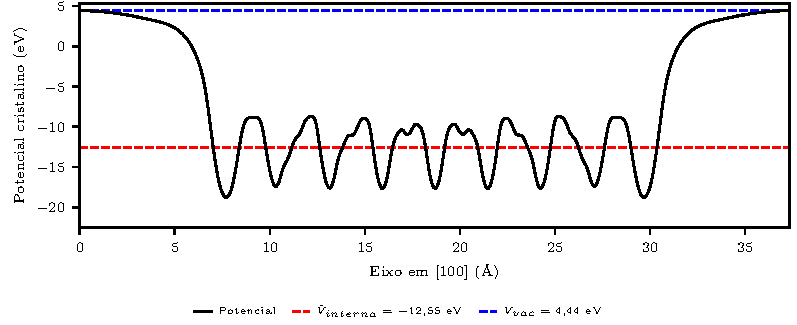
\includegraphics{../floats/vacuum_tf/x_potential.pdf}
    \end{figure}
\end{frame}